\documentclass{book}
\usepackage[a4paper,top=2.5cm,bottom=2.5cm,left=2.5cm,right=2.5cm]{geometry}
\usepackage{makeidx}
\usepackage{natbib}
\usepackage{graphicx}
\usepackage{multicol}
\usepackage{float}
\usepackage{listings}
\usepackage{color}
\usepackage{ifthen}
\usepackage[table]{xcolor}
\usepackage{textcomp}
\usepackage{alltt}
\usepackage{ifpdf}
\ifpdf
\usepackage[pdftex,
            pagebackref=true,
            colorlinks=true,
            linkcolor=blue,
            unicode
           ]{hyperref}
\else
\usepackage[ps2pdf,
            pagebackref=true,
            colorlinks=true,
            linkcolor=blue,
            unicode
           ]{hyperref}
\usepackage{pspicture}
\fi
\usepackage[utf8]{inputenc}
\usepackage[spanish]{babel}
\usepackage{mathptmx}
\usepackage[scaled=.90]{helvet}
\usepackage{courier}
\usepackage{sectsty}
\usepackage{amssymb}
\usepackage[titles]{tocloft}
\usepackage{doxygen}
\lstset{language=C++,inputencoding=utf8,basicstyle=\footnotesize,breaklines=true,breakatwhitespace=true,tabsize=2,numbers=left }
\makeindex
\setcounter{tocdepth}{3}
\renewcommand{\footrulewidth}{0.4pt}
\renewcommand{\familydefault}{\sfdefault}
\hfuzz=15pt
\setlength{\emergencystretch}{15pt}
\hbadness=750
\tolerance=750
\begin{document}
\hypersetup{pageanchor=false,citecolor=blue}
\begin{titlepage}
\vspace*{7cm}
\begin{center}
{\Large Practica P\-R\-O2 \\[1ex]\large version 1 10-\/abr-\/2012 }\\
\vspace*{1cm}
{\large Generado por Doxygen 1.8.2}\\
\vspace*{0.5cm}
{\small Jueves, 24 de Abril de 2014 10:40:30}\\
\end{center}
\end{titlepage}
\clearemptydoublepage
\pagenumbering{roman}
\tableofcontents
\clearemptydoublepage
\pagenumbering{arabic}
\hypersetup{pageanchor=true,citecolor=blue}
\chapter{Índice de clases}
\section{Lista de clases}
Lista de las clases, estructuras, uniones e interfaces con una breve descripción\-:\begin{DoxyCompactList}
\item\contentsline{section}{\hyperlink{class_cjt__organismes}{Cjt\-\_\-organismes} \\*Conté un conjunt d'organismes }{\pageref{class_cjt__organismes}}{}
\item\contentsline{section}{\hyperlink{class_organisme}{Organisme} \\*Contiene celulas ordenadas }{\pageref{class_organisme}}{}
\end{DoxyCompactList}

\chapter{Indice de archivos}
\section{Lista de archivos}
Lista de todos los archivos con descripciones breves\-:\begin{DoxyCompactList}
\item\contentsline{section}{\hyperlink{_lista_palabras_8hpp}{Lista\-Palabras.\-hpp} \\*Especificación de la clase \hyperlink{class_lista_palabras}{Lista\-Palabras} }{\pageref{_lista_palabras_8hpp}}{}
\item\contentsline{section}{\hyperlink{_palabra_8hpp}{Palabra.\-hpp} \\*Especificación de la clase \hyperlink{class_palabra}{Palabra} }{\pageref{_palabra_8hpp}}{}
\item\contentsline{section}{\hyperlink{pro2__s52_8cpp}{pro2\-\_\-s52.\-cpp} \\*Programa principal para el ejercicio {\itshape Factor Psi} }{\pageref{pro2__s52_8cpp}}{}
\end{DoxyCompactList}

\chapter{Documentación de las clases}
\hypertarget{class_cjt__organismes}{\section{Referencia de la Clase Cjt\-\_\-organismes}
\label{class_cjt__organismes}\index{Cjt\-\_\-organismes@{Cjt\-\_\-organismes}}
}


conté un conjunt d'organismes  


\subsection*{Métodos públicos}
\begin{DoxyCompactItemize}
\item 
\hyperlink{class_cjt__organismes_aeef5a3310bf21961ed1976585c531a75}{Cjt\-\_\-organismes} (int M)
\begin{DoxyCompactList}\small\item\em Creadora por defecto. \end{DoxyCompactList}\item 
\hyperlink{class_cjt__organismes_ae4c9a822f84e06f17f3e58c0747fd2ff}{$\sim$\-Cjt\-\_\-organismes} ()
\item 
void \hyperlink{class_cjt__organismes_a32f1d55b2e11f6f724e22f305712d3a1}{estiron\-\_\-id} ()
\begin{DoxyCompactList}\small\item\em realiza el estiron a partir de una secuencia de entrada \end{DoxyCompactList}\item 
bool \hyperlink{class_cjt__organismes_a33b52c7d797c0ee244e3c77cb4d2b86e}{recorte\-\_\-id} ()
\begin{DoxyCompactList}\small\item\em realiza un recorte a partir de una secuencia de entrada \end{DoxyCompactList}\item 
bool \hyperlink{class_cjt__organismes_ab6061ae3fc10ae709a2584335e687271}{ronda} ()
\begin{DoxyCompactList}\small\item\em realiza una ronda de reproducción a todos los organismos \end{DoxyCompactList}\item 
void \hyperlink{class_cjt__organismes_a0c8bed8ae75e0d8ff377be4ca1ee05bc}{consult\-\_\-id} ()
\begin{DoxyCompactList}\small\item\em Consultora estados de los subconjuntos segun una secuencia de entrada. \end{DoxyCompactList}\item 
void \hyperlink{class_cjt__organismes_a572fa37acffaf39795c0a4af932a96b6}{consult\-\_\-round} ()
\begin{DoxyCompactList}\small\item\em Consultora del estado de los organismos nacidos en la ultima ronda. \end{DoxyCompactList}\item 
void \hyperlink{class_cjt__organismes_a92aaf8ea473cf2c96691dc729d953baa}{consult\-\_\-ranking\-\_\-rep} ()
\begin{DoxyCompactList}\small\item\em Consultora de ranking de reproducción. \end{DoxyCompactList}\item 
void \hyperlink{class_cjt__organismes_ad68c53287bf354d7dc5efd78266b76fc}{leer\-\_\-cjt} (int n, int M)
\begin{DoxyCompactList}\small\item\em Operación de lectura. \end{DoxyCompactList}\end{DoxyCompactItemize}


\subsection{Descripción detallada}
conté un conjunt d'organismes 

Definición en la línea 15 del archivo Cjt\-\_\-organismes.\-hpp.



\subsection{Documentación del constructor y destructor}
\hypertarget{class_cjt__organismes_aeef5a3310bf21961ed1976585c531a75}{\index{Cjt\-\_\-organismes@{Cjt\-\_\-organismes}!Cjt\-\_\-organismes@{Cjt\-\_\-organismes}}
\index{Cjt\-\_\-organismes@{Cjt\-\_\-organismes}!Cjt_organismes@{Cjt\-\_\-organismes}}
\subsubsection[{Cjt\-\_\-organismes}]{\setlength{\rightskip}{0pt plus 5cm}Cjt\-\_\-organismes\-::\-Cjt\-\_\-organismes (
\begin{DoxyParamCaption}
\item[{int}]{M}
\end{DoxyParamCaption}
)}}\label{class_cjt__organismes_aeef5a3310bf21961ed1976585c531a75}


Creadora por defecto. 

Se ejecuta automáticamente al declarar una lavadora. \begin{DoxyPrecond}{Precondición}
cierto 
\end{DoxyPrecond}
\begin{DoxyPostcond}{Postcondición}
El resultado es un vector con M posiciones, con M organismos vacíos 
\end{DoxyPostcond}
\hypertarget{class_cjt__organismes_ae4c9a822f84e06f17f3e58c0747fd2ff}{\index{Cjt\-\_\-organismes@{Cjt\-\_\-organismes}!$\sim$\-Cjt\-\_\-organismes@{$\sim$\-Cjt\-\_\-organismes}}
\index{$\sim$\-Cjt\-\_\-organismes@{$\sim$\-Cjt\-\_\-organismes}!Cjt_organismes@{Cjt\-\_\-organismes}}
\subsubsection[{$\sim$\-Cjt\-\_\-organismes}]{\setlength{\rightskip}{0pt plus 5cm}Cjt\-\_\-organismes\-::$\sim$\-Cjt\-\_\-organismes (
\begin{DoxyParamCaption}
{}
\end{DoxyParamCaption}
)}}\label{class_cjt__organismes_ae4c9a822f84e06f17f3e58c0747fd2ff}


\subsection{Documentación de las funciones miembro}
\hypertarget{class_cjt__organismes_a32f1d55b2e11f6f724e22f305712d3a1}{\index{Cjt\-\_\-organismes@{Cjt\-\_\-organismes}!estiron\-\_\-id@{estiron\-\_\-id}}
\index{estiron\-\_\-id@{estiron\-\_\-id}!Cjt_organismes@{Cjt\-\_\-organismes}}
\subsubsection[{estiron\-\_\-id}]{\setlength{\rightskip}{0pt plus 5cm}void Cjt\-\_\-organismes\-::estiron\-\_\-id (
\begin{DoxyParamCaption}
{}
\end{DoxyParamCaption}
)}}\label{class_cjt__organismes_a32f1d55b2e11f6f724e22f305712d3a1}


realiza el estiron a partir de una secuencia de entrada 

\begin{DoxyPrecond}{Precondición}
cert 
\end{DoxyPrecond}
\begin{DoxyPostcond}{Postcondición}
se ha realizado el estiron a los id de la secuencia de entrada (si ha sido posible) 
\end{DoxyPostcond}
\hypertarget{class_cjt__organismes_a33b52c7d797c0ee244e3c77cb4d2b86e}{\index{Cjt\-\_\-organismes@{Cjt\-\_\-organismes}!recorte\-\_\-id@{recorte\-\_\-id}}
\index{recorte\-\_\-id@{recorte\-\_\-id}!Cjt_organismes@{Cjt\-\_\-organismes}}
\subsubsection[{recorte\-\_\-id}]{\setlength{\rightskip}{0pt plus 5cm}bool Cjt\-\_\-organismes\-::recorte\-\_\-id (
\begin{DoxyParamCaption}
{}
\end{DoxyParamCaption}
)}}\label{class_cjt__organismes_a33b52c7d797c0ee244e3c77cb4d2b86e}


realiza un recorte a partir de una secuencia de entrada 

\begin{DoxyPrecond}{Precondición}
cert 
\end{DoxyPrecond}
\begin{DoxyPostcond}{Postcondición}
se ha realizado el recorte a los id de la secuencia de entrada (si ha sido posible) si al acabar han muerto todos los organismos, escribira\-: \char`\"{}\-Han muerto todos los organismo. Fin del experimento\char`\"{} y devolverá true, si no devolvera false 
\end{DoxyPostcond}
\hypertarget{class_cjt__organismes_ab6061ae3fc10ae709a2584335e687271}{\index{Cjt\-\_\-organismes@{Cjt\-\_\-organismes}!ronda@{ronda}}
\index{ronda@{ronda}!Cjt_organismes@{Cjt\-\_\-organismes}}
\subsubsection[{ronda}]{\setlength{\rightskip}{0pt plus 5cm}bool Cjt\-\_\-organismes\-::ronda (
\begin{DoxyParamCaption}
{}
\end{DoxyParamCaption}
)}}\label{class_cjt__organismes_ab6061ae3fc10ae709a2584335e687271}


realiza una ronda de reproducción a todos los organismos 

\begin{DoxyPrecond}{Precondición}
cert 
\end{DoxyPrecond}
\begin{DoxyPostcond}{Postcondición}
se ha realizado una ronda de reproducción a todos los organismos, actualizado el ranking, y escribre el numero de hijos nacidos por el canal de salida estandar. Si numero de organismos llega a M, escribe \char`\"{}\-Población historica máxima alcanzada. Fin del experimento\char`\"{} en el canal de salida estandar y devuelve true. Si no devuelve false 
\end{DoxyPostcond}
\hypertarget{class_cjt__organismes_a0c8bed8ae75e0d8ff377be4ca1ee05bc}{\index{Cjt\-\_\-organismes@{Cjt\-\_\-organismes}!consult\-\_\-id@{consult\-\_\-id}}
\index{consult\-\_\-id@{consult\-\_\-id}!Cjt_organismes@{Cjt\-\_\-organismes}}
\subsubsection[{consult\-\_\-id}]{\setlength{\rightskip}{0pt plus 5cm}void Cjt\-\_\-organismes\-::consult\-\_\-id (
\begin{DoxyParamCaption}
{}
\end{DoxyParamCaption}
)}}\label{class_cjt__organismes_a0c8bed8ae75e0d8ff377be4ca1ee05bc}


Consultora estados de los subconjuntos segun una secuencia de entrada. 

\begin{DoxyPrecond}{Precondición}
cert 
\end{DoxyPrecond}
\begin{DoxyPostcond}{Postcondición}
escribe la estructura celular de los subconjuntos pedidos en el canal de salida estandar 
\end{DoxyPostcond}
\hypertarget{class_cjt__organismes_a572fa37acffaf39795c0a4af932a96b6}{\index{Cjt\-\_\-organismes@{Cjt\-\_\-organismes}!consult\-\_\-round@{consult\-\_\-round}}
\index{consult\-\_\-round@{consult\-\_\-round}!Cjt_organismes@{Cjt\-\_\-organismes}}
\subsubsection[{consult\-\_\-round}]{\setlength{\rightskip}{0pt plus 5cm}void Cjt\-\_\-organismes\-::consult\-\_\-round (
\begin{DoxyParamCaption}
{}
\end{DoxyParamCaption}
)}}\label{class_cjt__organismes_a572fa37acffaf39795c0a4af932a96b6}


Consultora del estado de los organismos nacidos en la ultima ronda. 

\begin{DoxyPrecond}{Precondición}
cierto 
\end{DoxyPrecond}
\begin{DoxyPostcond}{Postcondición}
escribe el estado de los organismos nacidos en la ultima ronda 
\end{DoxyPostcond}
\hypertarget{class_cjt__organismes_a92aaf8ea473cf2c96691dc729d953baa}{\index{Cjt\-\_\-organismes@{Cjt\-\_\-organismes}!consult\-\_\-ranking\-\_\-rep@{consult\-\_\-ranking\-\_\-rep}}
\index{consult\-\_\-ranking\-\_\-rep@{consult\-\_\-ranking\-\_\-rep}!Cjt_organismes@{Cjt\-\_\-organismes}}
\subsubsection[{consult\-\_\-ranking\-\_\-rep}]{\setlength{\rightskip}{0pt plus 5cm}void Cjt\-\_\-organismes\-::consult\-\_\-ranking\-\_\-rep (
\begin{DoxyParamCaption}
{}
\end{DoxyParamCaption}
)}}\label{class_cjt__organismes_a92aaf8ea473cf2c96691dc729d953baa}


Consultora de ranking de reproducción. 

\begin{DoxyPrecond}{Precondición}
cierto 
\end{DoxyPrecond}
\begin{DoxyPostcond}{Postcondición}
se ha hecho la escritura del ranking mediante la funcion de la clase ranking\-: escribir\-\_\-rank\-\_\-rep() 
\end{DoxyPostcond}
\hypertarget{class_cjt__organismes_ad68c53287bf354d7dc5efd78266b76fc}{\index{Cjt\-\_\-organismes@{Cjt\-\_\-organismes}!leer\-\_\-cjt@{leer\-\_\-cjt}}
\index{leer\-\_\-cjt@{leer\-\_\-cjt}!Cjt_organismes@{Cjt\-\_\-organismes}}
\subsubsection[{leer\-\_\-cjt}]{\setlength{\rightskip}{0pt plus 5cm}void Cjt\-\_\-organismes\-::leer\-\_\-cjt (
\begin{DoxyParamCaption}
\item[{int}]{n, }
\item[{int}]{M}
\end{DoxyParamCaption}
)}}\label{class_cjt__organismes_ad68c53287bf354d7dc5efd78266b76fc}


Operación de lectura. 

\begin{DoxyPrecond}{Precondición}
n$<$=M 
\end{DoxyPrecond}
\begin{DoxyPostcond}{Postcondición}
se han almacenado los organismos(tanto en ranking, como en el vector Cjt) leidos por el canal de entrada estandar 
\end{DoxyPostcond}


La documentación para esta clase fue generada a partir del siguiente fichero\-:\begin{DoxyCompactItemize}
\item 
\hyperlink{_cjt__organismes_8hpp}{Cjt\-\_\-organismes.\-hpp}\end{DoxyCompactItemize}

\hypertarget{class_organisme}{\section{Referencia de la Clase Organisme}
\label{class_organisme}\index{Organisme@{Organisme}}
}


Contiene celulas ordenadas.  


\subsection*{Métodos públicos}
\begin{DoxyCompactItemize}
\item 
\hyperlink{class_organisme_a86e18d319ceca9bb5fd43ac630c78b40}{Organisme} (int x)
\begin{DoxyCompactList}\small\item\em Creadora por defecto. \end{DoxyCompactList}\item 
\hyperlink{class_organisme_a55c9d7cbc9683970ad88455fdc3be7aa}{$\sim$\-Organisme} ()
\item 
\hyperlink{class_organisme}{Organisme} \hyperlink{class_organisme_a589195c1a83c096fcd7487a8b9a8a0a7}{reproduccion\-\_\-org} (const \hyperlink{class_organisme}{Organisme} \&o)
\begin{DoxyCompactList}\small\item\em realiza la reproduccion entre el parámetro implícito y otro organismo \end{DoxyCompactList}\item 
void \hyperlink{class_organisme_acdc2be53a7fabf324235c19b313bf662}{estiron} ()
\begin{DoxyCompactList}\small\item\em realiza un estiron en el parámetro implícito \end{DoxyCompactList}\item 
bool \hyperlink{class_organisme_a1f97e234776174573cfb761e7697dc37}{recorte} ()
\begin{DoxyCompactList}\small\item\em realiza un recorte \end{DoxyCompactList}\item 
bool \hyperlink{class_organisme_a6428a0fc8326f50acbdf24f6a134e60b}{muerto} ()
\begin{DoxyCompactList}\small\item\em Consultora de estado. \end{DoxyCompactList}\item 
bool \hyperlink{class_organisme_a22b9c9694a3ffcb42314f29dd56a43a5}{estirable} ()
\begin{DoxyCompactList}\small\item\em Consultora de flexibilidad. \end{DoxyCompactList}\item 
void \hyperlink{class_organisme_aa8ef449b54a88d0073f9a5343e5a8441}{leer\-\_\-organismo} ()
\begin{DoxyCompactList}\small\item\em Operación de lectura. \end{DoxyCompactList}\item 
void \hyperlink{class_organisme_a5c72bf91508e29c1135b24e1d61bb335}{escriure\-\_\-organismo} ()
\begin{DoxyCompactList}\small\item\em Operación de escritura. \end{DoxyCompactList}\end{DoxyCompactItemize}


\subsection{Descripción detallada}
Contiene celulas ordenadas. 

Definición en la línea 14 del archivo Organisme.\-hpp.



\subsection{Documentación del constructor y destructor}
\hypertarget{class_organisme_a86e18d319ceca9bb5fd43ac630c78b40}{\index{Organisme@{Organisme}!Organisme@{Organisme}}
\index{Organisme@{Organisme}!Organisme@{Organisme}}
\subsubsection[{Organisme}]{\setlength{\rightskip}{0pt plus 5cm}Organisme\-::\-Organisme (
\begin{DoxyParamCaption}
\item[{int}]{x}
\end{DoxyParamCaption}
)}}\label{class_organisme_a86e18d319ceca9bb5fd43ac630c78b40}


Creadora por defecto. 

Se ejecuta automáticamente al declarar una cubeta. \begin{DoxyPrecond}{Precondición}
cierto 
\end{DoxyPrecond}
\begin{DoxyPostcond}{Postcondición}
El resultado es un organismo con I\-D=x muerto 
\end{DoxyPostcond}
\hypertarget{class_organisme_a55c9d7cbc9683970ad88455fdc3be7aa}{\index{Organisme@{Organisme}!$\sim$\-Organisme@{$\sim$\-Organisme}}
\index{$\sim$\-Organisme@{$\sim$\-Organisme}!Organisme@{Organisme}}
\subsubsection[{$\sim$\-Organisme}]{\setlength{\rightskip}{0pt plus 5cm}Organisme\-::$\sim$\-Organisme (
\begin{DoxyParamCaption}
{}
\end{DoxyParamCaption}
)}}\label{class_organisme_a55c9d7cbc9683970ad88455fdc3be7aa}


\subsection{Documentación de las funciones miembro}
\hypertarget{class_organisme_a589195c1a83c096fcd7487a8b9a8a0a7}{\index{Organisme@{Organisme}!reproduccion\-\_\-org@{reproduccion\-\_\-org}}
\index{reproduccion\-\_\-org@{reproduccion\-\_\-org}!Organisme@{Organisme}}
\subsubsection[{reproduccion\-\_\-org}]{\setlength{\rightskip}{0pt plus 5cm}{\bf Organisme} Organisme\-::reproduccion\-\_\-org (
\begin{DoxyParamCaption}
\item[{const {\bf Organisme} \&}]{o}
\end{DoxyParamCaption}
)}}\label{class_organisme_a589195c1a83c096fcd7487a8b9a8a0a7}


realiza la reproduccion entre el parámetro implícito y otro organismo 

\begin{DoxyPrecond}{Precondición}
el organismo del parámetro implícito y o són compatibles, Cjt\-\_\-organismes.\-size()$<$M 
\end{DoxyPrecond}
\begin{DoxyPostcond}{Postcondición}
Crea un organismo con id=numero organismos+1 formado por la intersección de ambos más las celulas activas y actualiza numero organismos 
\end{DoxyPostcond}
\hypertarget{class_organisme_acdc2be53a7fabf324235c19b313bf662}{\index{Organisme@{Organisme}!estiron@{estiron}}
\index{estiron@{estiron}!Organisme@{Organisme}}
\subsubsection[{estiron}]{\setlength{\rightskip}{0pt plus 5cm}void Organisme\-::estiron (
\begin{DoxyParamCaption}
{}
\end{DoxyParamCaption}
)}}\label{class_organisme_acdc2be53a7fabf324235c19b313bf662}


realiza un estiron en el parámetro implícito 

\begin{DoxyPrecond}{Precondición}
el parámetro implícito es estirable 
\end{DoxyPrecond}
\begin{DoxyPostcond}{Postcondición}
El parámetro implícito pasa a ser el mismo, más la fisión de sus celulas sin hijos. 
\end{DoxyPostcond}
\hypertarget{class_organisme_a1f97e234776174573cfb761e7697dc37}{\index{Organisme@{Organisme}!recorte@{recorte}}
\index{recorte@{recorte}!Organisme@{Organisme}}
\subsubsection[{recorte}]{\setlength{\rightskip}{0pt plus 5cm}bool Organisme\-::recorte (
\begin{DoxyParamCaption}
{}
\end{DoxyParamCaption}
)}}\label{class_organisme_a1f97e234776174573cfb761e7697dc37}


realiza un recorte 

\begin{DoxyPrecond}{Precondición}
El parámetro implícito no está muerto 
\end{DoxyPrecond}
\begin{DoxyPostcond}{Postcondición}
El parámetro implícito pasa a ser el mismo, menos las celulas sin hijos, devuelve true si el organismo ha muerto, false si sigue vivo 
\end{DoxyPostcond}
\hypertarget{class_organisme_a6428a0fc8326f50acbdf24f6a134e60b}{\index{Organisme@{Organisme}!muerto@{muerto}}
\index{muerto@{muerto}!Organisme@{Organisme}}
\subsubsection[{muerto}]{\setlength{\rightskip}{0pt plus 5cm}bool Organisme\-::muerto (
\begin{DoxyParamCaption}
{}
\end{DoxyParamCaption}
)}}\label{class_organisme_a6428a0fc8326f50acbdf24f6a134e60b}


Consultora de estado. 

\begin{DoxyPrecond}{Precondición}
cierto 
\end{DoxyPrecond}
\begin{DoxyPostcond}{Postcondición}
El resultado es cierto si el organismo ha perdido la celula madre, falso si no la ha perdido 
\end{DoxyPostcond}
\hypertarget{class_organisme_a22b9c9694a3ffcb42314f29dd56a43a5}{\index{Organisme@{Organisme}!estirable@{estirable}}
\index{estirable@{estirable}!Organisme@{Organisme}}
\subsubsection[{estirable}]{\setlength{\rightskip}{0pt plus 5cm}bool Organisme\-::estirable (
\begin{DoxyParamCaption}
{}
\end{DoxyParamCaption}
)}}\label{class_organisme_a22b9c9694a3ffcb42314f29dd56a43a5}


Consultora de flexibilidad. 

\begin{DoxyPrecond}{Precondición}
el parámetro implícito no está muerto 
\end{DoxyPrecond}
\begin{DoxyPostcond}{Postcondición}
El resultado es cierto si hay celulas fisionables, falso si no 
\end{DoxyPostcond}
\hypertarget{class_organisme_aa8ef449b54a88d0073f9a5343e5a8441}{\index{Organisme@{Organisme}!leer\-\_\-organismo@{leer\-\_\-organismo}}
\index{leer\-\_\-organismo@{leer\-\_\-organismo}!Organisme@{Organisme}}
\subsubsection[{leer\-\_\-organismo}]{\setlength{\rightskip}{0pt plus 5cm}void Organisme\-::leer\-\_\-organismo (
\begin{DoxyParamCaption}
{}
\end{DoxyParamCaption}
)}}\label{class_organisme_aa8ef449b54a88d0073f9a5343e5a8441}


Operación de lectura. 

\begin{DoxyPrecond}{Precondición}
el organismo tiene almenos una celula 
\end{DoxyPrecond}
\begin{DoxyPostcond}{Postcondición}
el parámetro implícito pasa a tener el organismo descrito en el canal de entrada 
\end{DoxyPostcond}
\hypertarget{class_organisme_a5c72bf91508e29c1135b24e1d61bb335}{\index{Organisme@{Organisme}!escriure\-\_\-organismo@{escriure\-\_\-organismo}}
\index{escriure\-\_\-organismo@{escriure\-\_\-organismo}!Organisme@{Organisme}}
\subsubsection[{escriure\-\_\-organismo}]{\setlength{\rightskip}{0pt plus 5cm}void Organisme\-::escriure\-\_\-organismo (
\begin{DoxyParamCaption}
{}
\end{DoxyParamCaption}
)}}\label{class_organisme_a5c72bf91508e29c1135b24e1d61bb335}


Operación de escritura. 

\begin{DoxyPrecond}{Precondición}
cierto 
\end{DoxyPrecond}
\begin{DoxyPostcond}{Postcondición}
Escribe el contenido del parámetro implícito por el canal estándar de salida 
\end{DoxyPostcond}


La documentación para esta clase fue generada a partir del siguiente fichero\-:\begin{DoxyCompactItemize}
\item 
\hyperlink{_organisme_8hpp}{Organisme.\-hpp}\end{DoxyCompactItemize}

\chapter{Documentación de archivos}
\hypertarget{_cjt__organismes_8hpp}{\section{Referencia del Archivo Cjt\-\_\-organismes.\-hpp}
\label{_cjt__organismes_8hpp}\index{Cjt\-\_\-organismes.\-hpp@{Cjt\-\_\-organismes.\-hpp}}
}


Especificación de la clase \hyperlink{_cjt__organismes_8hpp}{Cjt\-\_\-organismes.\-hpp}.  


Dependencia gráfica adjunta para Cjt\-\_\-organismes.\-hpp\-:
\nopagebreak
\begin{figure}[H]
\begin{center}
\leavevmode
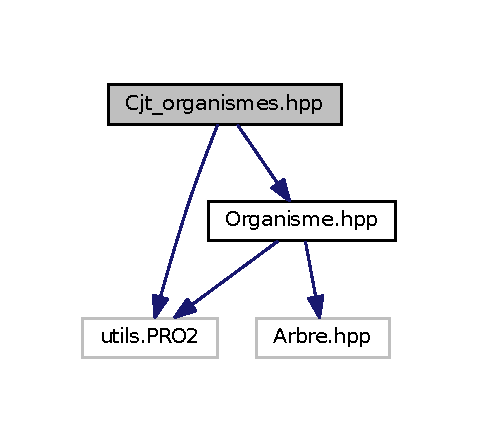
\includegraphics[width=278pt]{_cjt__organismes_8hpp__incl}
\end{center}
\end{figure}
\subsection*{Clases}
\begin{DoxyCompactItemize}
\item 
class \hyperlink{class_cjt__organismes}{Cjt\-\_\-organismes}
\begin{DoxyCompactList}\small\item\em conté un conjunt d'organismes \end{DoxyCompactList}\end{DoxyCompactItemize}


\subsection{Descripción detallada}
Especificación de la clase \hyperlink{_cjt__organismes_8hpp}{Cjt\-\_\-organismes.\-hpp}. 

Definición en el archivo \hyperlink{_cjt__organismes_8hpp_source}{Cjt\-\_\-organismes.\-hpp}.


\hypertarget{_organisme_8hpp}{\section{Referencia del Archivo Organisme.\-hpp}
\label{_organisme_8hpp}\index{Organisme.\-hpp@{Organisme.\-hpp}}
}


Especificación de la clase \hyperlink{class_organisme}{Organisme}.  


Dependencia gráfica adjunta para Organisme.\-hpp\-:
\nopagebreak
\begin{figure}[H]
\begin{center}
\leavevmode
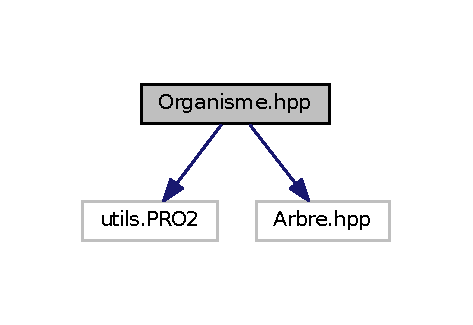
\includegraphics[width=227pt]{_organisme_8hpp__incl}
\end{center}
\end{figure}
\subsection*{Clases}
\begin{DoxyCompactItemize}
\item 
class \hyperlink{class_organisme}{Organisme}
\begin{DoxyCompactList}\small\item\em Contiene celulas ordenadas. \end{DoxyCompactList}\end{DoxyCompactItemize}


\subsection{Descripción detallada}
Especificación de la clase \hyperlink{class_organisme}{Organisme}. 

Definición en el archivo \hyperlink{_organisme_8hpp_source}{Organisme.\-hpp}.


\addcontentsline{toc}{part}{Índice}
\printindex
\end{document}
